%-*- coding:utf-8 -*-

\documentclass[10pt,dvipdfmx]{beamer}
\usepackage{tutorial}

\title{計算機実験II (L3) --- 量子力学}
\date{2020/10/16}

\begin{document}

\begin{frame}
  \titlepage
  \tableofcontents
\end{frame}

\begin{frame}[t]{講義日程}
  \begin{itemize}
    % \setlength{\itemsep}{1em}
  \item 全8回 (金曜5限 {\color{red}17:05}-18:35)
    \begin{itemize}
    \item {\color{gray} 10月8日 第1回: 乱択アルゴリズム、モンテカルロ法}
    \item 10月15日 第2回: 多体系の統計力学、マルコフ連鎖モンテカルロ法
    \item 10月22日 第3回
    \item 10月29日 第4回
    \item 11月5日 休講 (もくもく会)
    \item 11月12日 休講 (物理学教室コロキウム)
    \item 11月19日 第5回
    \item 11月26日 休講 (物理学教室コロキウム)
    \item 12月3日 第6回
    \item 12月10日 第7回
    \item 12月17日 休講 (物理学教室コロキウム)
    \item 12月24日 第8回
    \item 1月7日 休講 (もくもく会)
    \item 1月18日(火) 休講 (予備日)
    \end{itemize}
  \end{itemize}
\end{frame}


\section{シュレディンガー方程式の固有値問題 (復習)}
\begin{frame}[t,fragile]{時間依存しないシュレディンガー方程式}
  \begin{itemize}
    \setlength{\itemsep}{1em}
  \item 井戸型ポテンシャル中の一粒子問題
    \begin{align*}
      \big[ -\frac{\hbar^2}{2m}\frac{d^2}{dx^2} + V(x) \big] \psi(x) = E \psi(x) \\
      V(x) = \begin{cases}
        0 & \text{$a \le x \le b$} \\ \infty & \text{otherwise}
      \end{cases}
    \end{align*}
  \item $\hbar^2/2m = 1$、$a=0$、$b=1$となるように変数変換して
    \begin{align*}
      \big( \frac{d^2}{dx^2} + E \big) \psi(x) = 0 \qquad 0 \le x \le 1
    \end{align*}
    を境界条件$\psi(0) = \psi(1) = 0$のもとで解けば良い
  \end{itemize}
\end{frame}

\begin{frame}[t,fragile]{固有値問題の解法}
  \begin{itemize}
    \setlength{\itemsep}{1em}
  \item $x_i=h \times i$ ($h=1/n$)、$x_0=0$、$x_n=1$とする
  \item $\psi(x_0)=0$、$\psi(x_1) = 1$を仮定 ($\psi'(x_0)=1/h$と与えたことに相当)
  \item $E = 0$とおく
  \item Runge-Kutta法、Numerov法などを用いて$x=x_n$まで積分
  \item $\psi(x_n)$の符号がかわるまで、$E$を少しずつ増やす
  \item 符号が変わったら、$E$の区間を半分ずつに狭めていき、$\psi(x_n)=0$となる$E$ (固有エネルギー)と$\psi(x)$ (波動関数)を得る
  \end{itemize}
\end{frame}

\begin{frame}[t,fragile]{シュレディンガー方程式の行列表示}
  \begin{itemize}
    %\setlength{\itemsep}{1em}
  \item シュレディンガー方程式
    \[
    [-\frac{d^2}{dx^2}+V(x)]\psi(x) = E \psi(x)
    \]
  \item 連立差分方程式を行列の形で表す($\psi(x_0)=\psi(x_n)=0$)
    \begin{footnotesize}
    \[
    \begin{pmatrix}
      \frac{2}{h^2}+V(x_1) & -\frac{1}{h^2} \\
      -\frac{1}{h^2} & \frac{2}{h^2}+V(x_2) & -\frac{1}{h^2} \\
      & -\frac{1}{h^2} & \frac{2}{h^2}+V(x_3) & -\frac{1}{h^2} \\
      & & \ddots & \ddots \\
      & & & -\frac{1}{h^2} & \frac{2}{h^2}+V(x_{n-1}) \\
    \end{pmatrix}
    \begin{pmatrix}
      \psi(x_1) \\
      \psi(x_2) \\
      \psi(x_3) \\
      \vdots \\
      \psi(x_{n-1}) \\
    \end{pmatrix}
    = \cdots % E
    %% \begin{pmatrix}
    %%   \psi(x_1) \\
    %%   \psi(x_2) \\
    %%   \psi(x_3) \\
    %%   \vdots \\
    %%   \psi(x_{n-1}) \\
    %% \end{pmatrix}
    \]
    \end{footnotesize}
  \item $(n-1) \times (n-1)$の疎行列の固有値問題
    \begin{itemize}
    \item 固有値: 固有エネルギー
    \item 固有ベクトル: 波動関数
    \end{itemize}
  \end{itemize}
\end{frame}


%-*- coding:utf-8 -*-

\begin{frame}[t,fragile]{変分法}
  \begin{itemize}
    %\setlength{\itemsep}{1em}
  \item 波動関数を互いに直交する正規化された波動関数(基底関数)の線形結合で近似する (変分波動関数、試行関数)
    \begin{align*}
      | \psi \rangle = \sum_{p=1}^m C_p | \phi_p \rangle \qquad (\langle \phi_p | \phi_q \rangle = \delta_{pq})
    \end{align*}
  \item エネルギーの期待値
    \begin{align*}
      E &= \frac{\langle \psi | H | \psi \rangle}{\langle \psi | \psi \rangle} = \frac{\sum_{p,q} C_p^* H_{pq} C_q}{\sum_{p,q} C_p^* \delta_{pq} C_q} \\
      H_{pq} &= \langle \phi_p | H | \phi_q \rangle
    \end{align*}
  \item $E$ができるだけ小さくなるよう係数$C_p$を最適化 (変分原理)
  \end{itemize}
\end{frame}

%-*- coding:utf-8 -*-

\begin{frame}[t,fragile]{変分法}
  \begin{itemize}
    %\setlength{\itemsep}{1em}
  \item $\delta E = 0$から
    \begin{align*}
      \sum_{q} (H_{pq} - E \delta_{pq} ) C_q = 0 \qquad \text{for $^\forall p$}
    \end{align*}
  \item $H_{pq}$, $\delta_{pq}$を$m \times m$行列と考えると、固有値問題とみなせる
    \begin{align*}
      H C = E C
    \end{align*}
  \item $H$はエルミート行列
  \item $\{ \phi_p \}$の張る部分空間での最適化 (= Rayleigh-Ritzの方法)
  \item 変分波動関数と真の波動関数の差が$\epsilon$程度の時、$E$と真の固有エネルギーの差は$\epsilon^2$程度
  \end{itemize}
\end{frame}

%-*- coding:utf-8 -*-

\begin{frame}[t,fragile]{非直交基底関数による変分法}
  \begin{itemize}
    %\setlength{\itemsep}{1em}
  \item 重なり積分
    \begin{align*}
      S_{pq} = \langle \phi_p | \phi_q \rangle \ne \delta_{pq}
    \end{align*}
  \item 変分波動関数の正規化条件
    \begin{align*}
      \langle \psi | \psi \rangle = \sum_{p,q} C_p^* \langle \phi_p | \phi_q \rangle C_q = \sum_{p,q} C_p^* S_{pq} C_q = 1
    \end{align*}
  \item エネルギー期待値
    \begin{align*}
      E = \frac{\sum_{p,q} C_p^* H_{pq} C_q}{\sum_{p,q} C_p^* S_{pq} C_q}
    \end{align*}
  \item $\delta E = 0$から
    \begin{align*}
      \sum_q (H_{pq} - E S_{pq}) C_q = 0 \ \Rightarrow \ HC = ESC \ \text{(一般化固有値問題)}
    \end{align*}
  \end{itemize}
\end{frame}


\section{偏微分方程式の境界値問題 (復習)}

\begin{frame}[t,fragile]{ポアソン方程式の境界値問題}
  \begin{itemize}
    %\setlength{\itemsep}{1em}
  \item 二次元ポアソン方程式
    \[ \frac{\partial^2 u(x,y)}{\partial x^2} + \frac{\partial^2 u(x,y)}{\partial y^2} = f(x,y) \qquad 0 \le x \le 1, \ 0 \le y \le 1\]
  \item ディリクレ型境界条件: $u(x,y) = g(x,y)$ on $\partial \Omega$
  \item 有限差分法により離散化
    \begin{itemize}
    \item $x$方向、$y$方向をそれぞれ$n$等分: $(x_i,y_j) = (i/n, j/n)$
    \item $(n+1)^2$個の格子点の上で$u(x_i,y_j)=u_{ij}$が定義される
    \item そのうち$4n$個の値は境界条件で定まる
    \item ポアソン方程式を中心差分で近似 ($h=1/n$)
      \[
      \frac{u_{i+1,j}-2u_{ij}+u_{i-1,j}}{h^2} + \frac{u_{i,j+1}-2u_{ij}+u_{i,j-1}}{h^2} = f_{ij}
      \]
      残り$(n-1)^2$個の未知数に対する連立一次方程式
    \end{itemize}
  \end{itemize}
\end{frame}


%\section{偏微分方程式の初期値問題}
%-*- coding:utf-8 -*-

\section{偏微分方程式の初期値問題}

\begin{frame}[t]{一次元拡散方程式(放物型)}
  \begin{itemize}
  \item 一次元拡散方程式: $u=u(x,t)$, $q=q(x,t)$
    \[
    \frac{\partial u}{\partial t} - D \frac{\partial^2 u}{\partial x^2} = q
    \]
    \begin{itemize}
    \item 初期条件: $u(x,0) = f(x)$
    \item 境界条件: $u(0,t) = u(1,t) = 0$
    \end{itemize}
  \item 時間$t$と位置$x$に関して離散化
    \begin{align*}
      & u_j^n = u(x_j, t_n) \\
      & q_j^n = q(x_j, t_n) \\
      & t_0 = 0, t_1=\Delta t, t_2=2 \Delta t, \cdots, t_n=n \Delta t, \cdots \\
      & x_0 = 0, x_1=\Delta x, x_2=2 \Delta x, \cdots, x_N=N \Delta x = 1 \qquad (\Delta x = 1/N)
    \end{align*}
  \end{itemize}
\end{frame}

\begin{frame}[t]{有限差分法}
  \begin{itemize}
  \item $t$に関して前進差分を考える
    \[
    \frac{\partial u}{\partial t} \Big|_{(j \Delta x, n \Delta t)} = \frac{u_j^{n+1} - u_j^n}{\Delta t} + {\cal O}(\Delta t)
    \]
  \item $x$に関しては中心差分を考える
    \[
    \frac{\partial^2 u}{\partial x^2} \Big|_{(j \Delta x, n \Delta t)} = \frac{u_{j+1}^{n} - 2 u_{j}^{n} + u_{j-1}^{n}}{\Delta x^2} + {\cal O}(\Delta x^2)
    \]
  \item 拡散方程式に代入して整理すると
    \[
    u_{j}^{n+1} = u_{j}^{n} + r (u_{j+1}^{n} - 2 u_{j}^{n} + u_{j-1}^{n}) + \Delta t q_{j}^{n} \qquad (r = D\frac{\Delta t}{\Delta x^2})
    \]
  \item FTCS (Forward-Time Centered Space)法
  \end{itemize}
\end{frame}

\begin{frame}[t]{FTCS法}
  \begin{itemize}
  \item $O(\Delta t) + O(\Delta x^2)$の陽解法
    \begin{center}
      \resizebox{0.4\textwidth}{!}{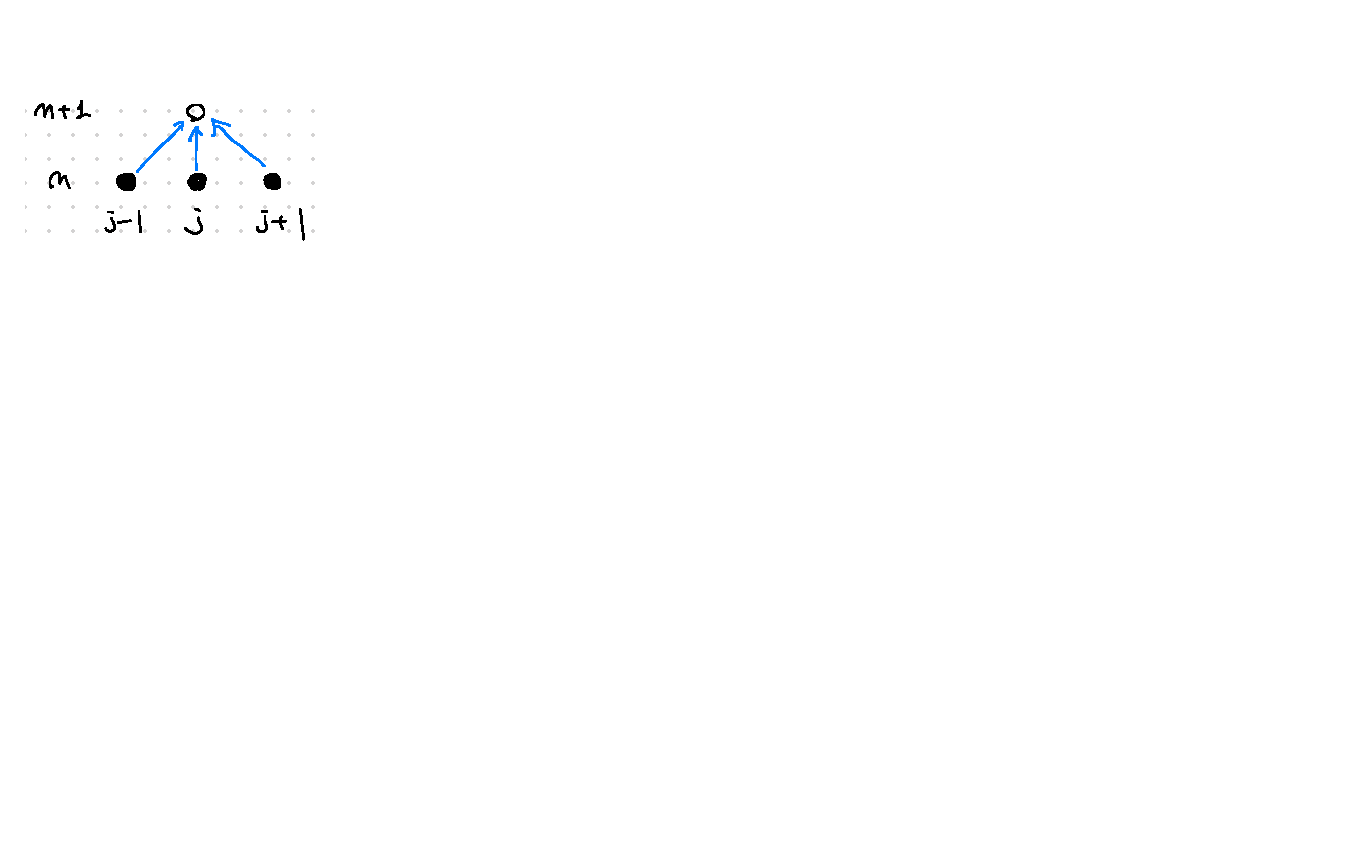
\includegraphics{image/ftcs-1.pdf}}
    \end{center}
  \item 初期条件
    \[
    u_j^0 = f(j\Delta x) \ \ (j=0,1,\cdots,N)
    \]
  \item 境界条件
    \[
    u_0^n = u_N^n = 0 \ \ (n=0,1,2,\cdots)
    \]
  \end{itemize}
\end{frame}

\begin{frame}[t]{有限差分法の安定性}
  \begin{itemize}
  \item (陽的)有限差分法においては、$\Delta t$、$\Delta x$は小さければ小さいほどよいというわけではない
  \item 一次元拡散方程式の場合
    \begin{align*}
      \begin{cases}
        r \le 1/2 & \text{安定} \\
        r > 1/2 & \text{\color{red}不安定}
      \end{cases}
    \end{align*}
  \item $\Delta x$を半分にしたら、$\Delta t$は1/4にしなければならない

    $\Rightarrow$ 計算量は8倍
  \end{itemize}
\end{frame}

\begin{frame}[t]{一次元波動方程式(双極型)}
  \begin{itemize}
  \item 一次元波動方程式
    \[
    \frac{\partial^2 u}{\partial t^2} = c^2 \frac{\partial^2 u}{\partial x^2} \qquad u(x,0)=f(x), \frac{\partial u}{\partial t} (x,0) = g(x)
    \]
  \item $t$に関する中心差分
    \[
    \frac{\partial^2 u}{\partial t^2} \Big|_{(j \Delta x, n \Delta t)} = \frac{u_{j}^{n+1} - 2 u_{j}^{n} + u_{j}^{n-1}}{\Delta t^2} + {\cal O}(\Delta t^2)
    \]
  \item 代入して整理すると
    \[
    u_{j}^{n+1} = 2u_{j}^{n} - u_{j}^{n-1} + \alpha^2 (u_{j+1}^{n} - 2 u_{j}^{n} + u_{j-1}^{n}) \qquad (\alpha = c\frac{\Delta t}{\Delta x})
    \]
  \end{itemize}
\end{frame}

\begin{frame}[t]{波動方程式に対するFTCS法}
  \begin{itemize}
  \item $O(\Delta t^2) + O(\Delta x^2)$の陽解法
    \begin{center}
      \resizebox{0.4\textwidth}{!}{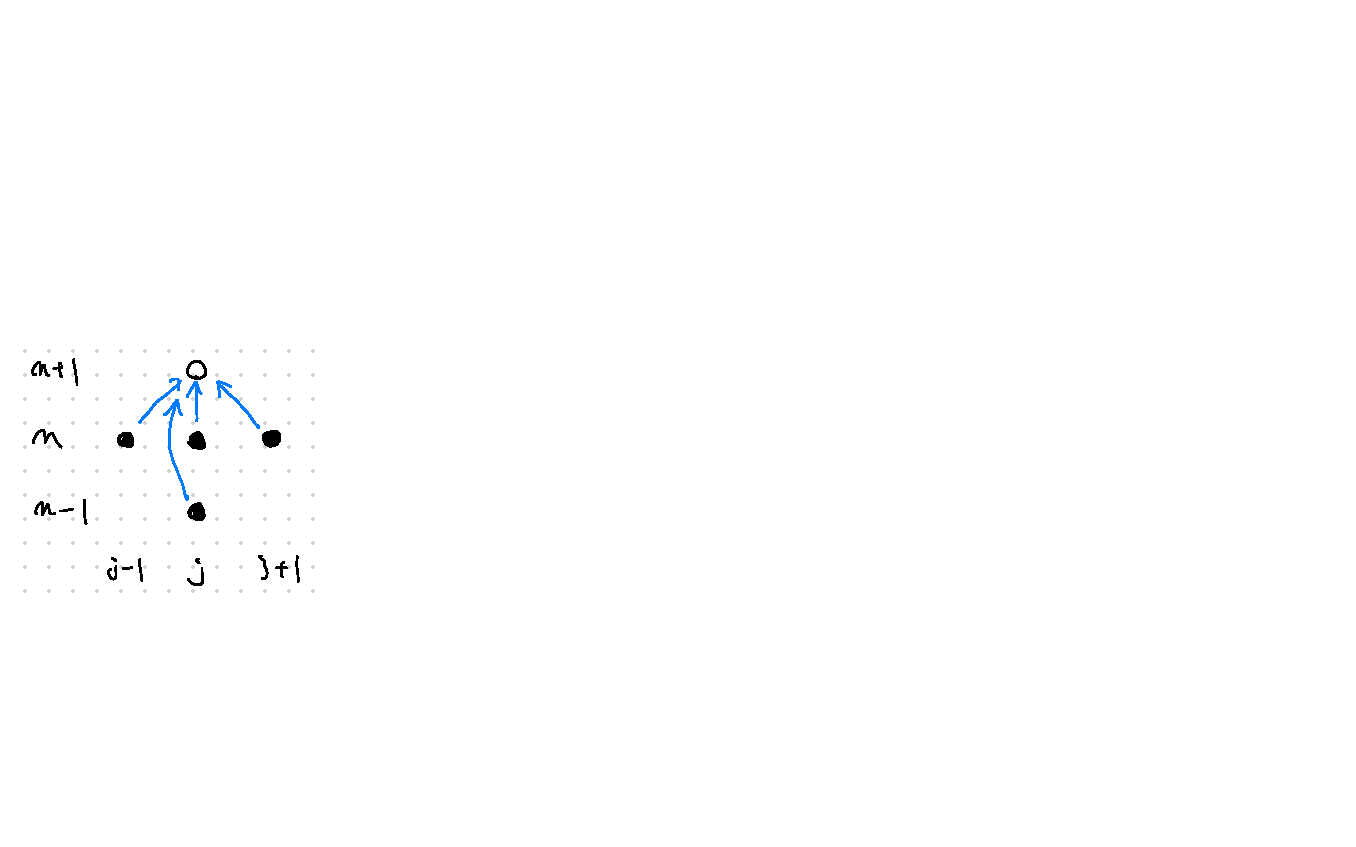
\includegraphics{image/ftcs-2.pdf}}
    \end{center}
  \item 初期条件
    \[
    u_j^0 = f(j\Delta x) \ \ (j=0,1,\cdots,N)
    \]
    初期速度については$n=0$に関する中心差分を考えて
    \[
    \frac{u_j^1 - u_j^{-1}}{2 \Delta t} = g_j \ \ \Rightarrow \ \ u_j^1 = u_j^0 + \Delta t g_j + \frac{\alpha^2}{2} (u_{j+1}^{n} - 2 u_{j}^{n} + u_{j-1}^{n})
    \]
  \end{itemize}
\end{frame}

\begin{frame}[t]{時間に依存するシュレディンガー方程式}
  \begin{itemize}
  \item 時間に依存するシュレディンガー方程式
    \[
    i \hbar \frac{\partial \Psi}{\partial t}(x,t) = H(x,t) \Psi(x,t) = \Big[ - \frac{\hbar^2}{2m} \frac{\partial^2}{\partial x^2} + V(x,t) \Big] \Psi(x,t)
    \]
    \begin{itemize}
    \item 波動関数のノルム $\displaystyle \int | \Psi(x,t) |^2 \, dx$ は保存
    \item $V(x,t)$が時間$t$に依存しない場合、エネルギーの期待値は保存
      \[
      \langle H \rangle = \frac{\displaystyle \int \Psi^* H \Psi \, dx}{\displaystyle \int | \Psi |^2 \, dx}
      \]
    \end{itemize}
  \item 以下では無次元化して$\hbar = m = 1$とおく
  \end{itemize}
\end{frame}

\begin{frame}[t]{時間に依存するシュレディンガー方程式}
  \begin{itemize}
  \item シュレディンガー方程式の形式解 ($V$が時間に依存しない場合)
    \[
    \Psi(x,t) = e^{-i H t} \Psi(x,0)
    \]
  \item $t$に関して前進差分
    \begin{align*}
      e^{-i H t} &= [e^{-i H \Delta t}]^M \approx [1 - i H \Delta t]^M \qquad (\Delta t = t / M) \\
      \Psi^{n+1} &= (1 -  i \Delta t H) \Psi^{n}
    \end{align*}
  \item $H$は対称(エルミート)行列 $\Rightarrow$ 時間発展演算子$e^{-i H \Delta t}$はユニタリー行列
  \item 差分近似$(1 -  i \Delta t H)$はユニタリーではない
    \begin{align*}
      & (e^{-i H \Delta t})^\dagger e^{-i H \Delta t} = e^{i H \Delta t} e^{-i H \Delta t} = 1 \\
      & (1 -  i \Delta t H)^\dagger (1 -  i \Delta t H) = (1 +  i \Delta t H) (1 -  i \Delta t H) = 1 + {\color{red} \Delta t^2 H^2}
    \end{align*}
  \end{itemize}
\end{frame}

\begin{frame}[t]{クランク・ニコルソン法}
  \begin{itemize}
  \item クランク・ニコルソン法
    \[
    \Psi^{n+1} = \frac{1 -  i \frac{\Delta t}{2} H}{1 +  i \frac{\Delta t}{2} H} \Psi^{n}
    \]
  \item (数値精度の範囲で)ユニタリー行列であるので、ノルムは保存
  \item $(1 +  i \frac{\Delta t}{2} H)^{-1}$を掛ける $\Rightarrow$ 連立一次方程式を解く必要がある
    \begin{itemize}
    \item まず、$\Psi = (1 - i \frac{\Delta t}{2} H) \Psi^n$ を計算
    \item 次に、$(1 +  i \frac{\Delta t}{2} H) \Psi^{n+1} = \Psi$ を解く(連立一次方程式)
    \end{itemize}
  \item 陰解法の一種
  \end{itemize}
\end{frame}

\begin{frame}[t]{陰解法}
  \begin{itemize}
  \item 時刻$t$関して後退差分を使う
    \[
    \frac{\partial u}{\partial t} \Big|_{(j \Delta x, n \Delta t)} = \frac{u_j^{n} - u_j^{n-1}}{\Delta t} + {\cal O}(\Delta t)
    \]
  \item $x$に関する中心差分と組み合わせ、$n \rightarrow n+1$と書き直すと
    \[
    u_{j}^{n+1} = u_{j}^{n} + r (u_{j+1}^{n+1} - 2 u_{j}^{n+1} + u_{j-1}^{n+1})
    \]
    $u^{n+1}$が両辺に現れる $\Rightarrow$ 陰解法
  \item $O(\Delta t) + O(\Delta x^2)$
  \item $r$の値によらず{\color{red}常に安定}
  \end{itemize}
\end{frame}

\begin{frame}[t]{クランク・ニコルソン法}
  \begin{itemize}
  \item さらに、時間方向にきざみ幅$\Delta t/2$の中心差分を使うと
    \[
    \frac{\partial u}{\partial t} \Big|_{(j \Delta x, n \Delta t)} = \frac{u_j^{n+\frac{1}{2}} - u_j^{n-\frac{1}{2}}}{\Delta t} + {\cal O}(\Delta t^2)
    \]
  \item $x$に関する中心差分と組み合わせ、$n \rightarrow n+\frac{1}{2}$し、さらに$u_j^{n+\frac{1}{2}}$を$(u_j^{n+1}+u_j^{n})/2$で近似すると
    \[
    u_{j}^{n+1} = u_{j}^{n} + \frac{r}{2} (u_{j+1}^{n+1} - 2 u_{j}^{n+1}  +u_{j-1}^{n+1} + u_{j+1}^{n} - 2 u_{j}^{n} + u_{j-1}^{n})
    \]
    あるいは
    \[
    u_{j}^{n+1} - \frac{r}{2} (u_{j+1}^{n+1} - 2 u_{j}^{n+1} + u_{j-1}^{n+1}) = u_{j}^{n} + \frac{r}{2} (u_{j+1}^{n} - 2 u_{j}^{n} + u_{j-1}^{n})
    \]
    $\Rightarrow$ クランク・ニコルソン法 [$O(\Delta t^2) + O(\Delta x^2)$]
  \end{itemize}
\end{frame}

%% \begin{frame}[t]{}
%%   \begin{itemize}
%%   \item
%%   \end{itemize}
%% \end{frame}


\section{}
\begin{frame}[t]{本日の課題}
  \begin{itemize}
    %\setlength{\itemsep}{1em}
  \item 実習
    \begin{itemize}
    \item 連立一次方程式の解法の復習 (計算機実験I 第5回)
    \item 実習課題一覧\href{https://github.com/todo-group/ComputerExperiments/releases/tag/2020a-computer2}{exercise-2.pdf}から偏微分方程式(あるいは別の)課題を選び実習
    \end{itemize}
  \item 質問はSlackの「\# 7\_偏微分方程式」あるいは他の適当と思われるチャンネルで
  \item 次回講義(10/23)の前日までにITC-LMSのアンケート「作業レポートNo.3」に回答
  \end{itemize}
\end{frame}

\end{document}
